%-----------------------------------------------%
% Modelo de Lista de Exercícios
%
% Autor: Rodrigo Nascimento (2022-08-12)
%-----------------------------------------------%

\documentclass[
	% -- opções da classe memoir --
	12pt,				% tamanho da fonte
	openright,			% capítulos começam em pág ímpar (insere página vazia caso preciso)
	oneside,			% twoside para impressão em verso e anverso. Oposto a oneside
	a4paper,			% tamanho do papel. 
	% -- opções da classe abntex2 --
	%chapter=TITLE,		% títulos de capítulos convertidos em letras maiúsculas
	%section=TITLE,		% títulos de seções convertidos em letras maiúsculas
	%subsection=TITLE,	% títulos de subseções convertidos em letras maiúsculas
	%subsubsection=TITLE,% títulos de subsubseções convertidos em letras maiúsculas
	% -- opções do pacote babel --
	english,			% idioma adicional para hifenização
%	french,				% idioma adicional para hifenização
%	spanish,			% idioma adicional para hifenização
	brazil				% o último idioma é o principal do documento
]{abntex2}
\selectlanguage{brazil}
%-----------------------------------------------%
% Informações do DOCUMENTO
%-----------------------------------------------%
\instituicao{Universidade do Estado de Santa Catarina -- UDESC}
\titulo{Notas de Mecânica Estatística}
\autor{Rodrigo Nascimento}
\local{Joinville - SC}
\data{\mydate}
\tipotrabalho{Nota de Aula:}
\orientador{Dr. Bruno Duarte da Silva Moreira}
\coorientador{Prof. Me. Supervisor}
%-----------------------------------------------%
% Para alterar o parâmetros dos comandos orientador
% e coorientador.
%-----------------------------------------------%
% \renewcommand{\orientadorname}{Orientadora:}
\renewcommand{\coorientadorname}{Supervisor:}
%-----------------------------------------------%

\newcommand{\centro}{Centro de Ciências Tecnológicas -- CCT }
\newcommand{\departamento}{Departamento de Física -- DFIS}
\newcommand{\curso}{Licenciatura em Física }
\newcommand{\disciplina}{Mecânica Estatística -- OMEE001}
\newcommand{\firstkey}{Introdução aos métodos estatísticos}
\newcommand{\secondkey}{Descrição estatística de sistemas físicos}
\newcommand{\thirdkey}{Termodinâmica}
\newcommand{\fourthkey}{Ensemble microcanônico}


%-----------------------------------------------%

% Todas as indicações de pacotes e configurações estão no arquivo de estilo
% chamado texmodel-udesc.sty.
\usepackage{texmodel-udesc}

%--------------------%
% Início do documento
%--------------------%
\begin{document}
% ---------------------------
% Insere o CABEÇALHO (HEADER)
% ---------------------------
    \thispagestyle{empty}
\begin{center}
	\begin{minipage}[!]{\linewidth}
        \begin{minipage}[!]{.19\linewidth}
            
\includegraphics[width=\linewidth]{img/logo.png}           
        \end{minipage}
        \begin{minipage}[!]{.8\linewidth}
            \center
            \ABNTEXchapterfont\normalsize\MakeUppercase{\imprimirinstituicao}
            \par
            \vspace*{3pt}                     
            \ABNTEXchapterfont\normalsize\MakeUppercase{\centro}
            \par
            \vspace*{3pt}
            \ABNTEXchapterfont\normalsize\MakeUppercase{\departamento}
            \par
            \vspace*{3pt}           
            \ABNTEXchapterfont\normalsize\MakeUppercase{\disciplina}
        \end{minipage}        
    \end{minipage}
    \par\vspace{0.5cm}
    \rule{\textwidth}{.5pt}   
\end{center}  
	% -----------------------------
% Insere CAMPO DE IDENTIFICAÇÃO
% -----------------------------   
\noindent \textbf{Aluno(a):} \imprimirautor
\par\noindent \textbf{Professor(a):} \imprimirorientador\hfill{}\textbf{Capítulo(s) Ref.:} VII/VIII  
\par\noindent \textbf{\imprimirtipotrabalho} 003  \hfill{}\textbf{Data:} \imprimirdata\hfill{}\textbf{Fase:} LEF102-08U
\rule{\textwidth}{.5pt}
\bigskip{}
\begin{center}
	\ABNTEXchapterfont\Large\MakeUppercase{\imprimirtitulo}
\end{center}

% Campo para OBERVAÇÕES
\noindent \textbf{Resumo:} Atividade avaliativa baseada no livro do Salinas \cite{SALINAS:2001} para a disciplina de Mecânica Estatística – OMEE001.

\par\noindent \textbf{Palavras chave:} \firstkey; \secondkey; \thirdkey; \fourthkey.
%% ============| INÍCIO |===================
% --------------| Q01 |--------------------
\addcontentsline{toc}{section}{Questão}
\begin{prob}
  Considere a distribuição Gaussiana:
  \begin{align}
    p(x)=\frac{1}{\sqrt{2\pi\sigma^2}}\mathrm{e}^{-\frac{1}{2}\left(\frac{x-\mu}{\sigma}\right)^2}
  \end{align}
  onde $\sigma$ é o desvio padrão e $\mu$ a média. Faça plots de $p(x)$ contra $x$ para:
  \begin{enumerate}[label=\alph *)]
    \item $\mu=0$ e $\sigma=0,1$
    \item $\mu=1$ e $\sigma=0,1$
    \item $\mu=0$ e $\sigma=1$
    \item $\mu=1$ e $\sigma=1$
  \end{enumerate}
  Comente a semelhança e diferença entre os casos.
  \newpage
  \begin{sol}
  \par\noindent As \autoref{fig:gaussianas-1} e \autoref{fig:gaussianas-2}, mostram os gráficos das distribuições gaussianas $p(x)$ cada qual com médias $\mu$ e desvios padrão $\sigma$ indicado.
      \begin{figure}[!htb]
      \centering
      \subfloat[$\mu=0$ \label{fig:figura01}]{
        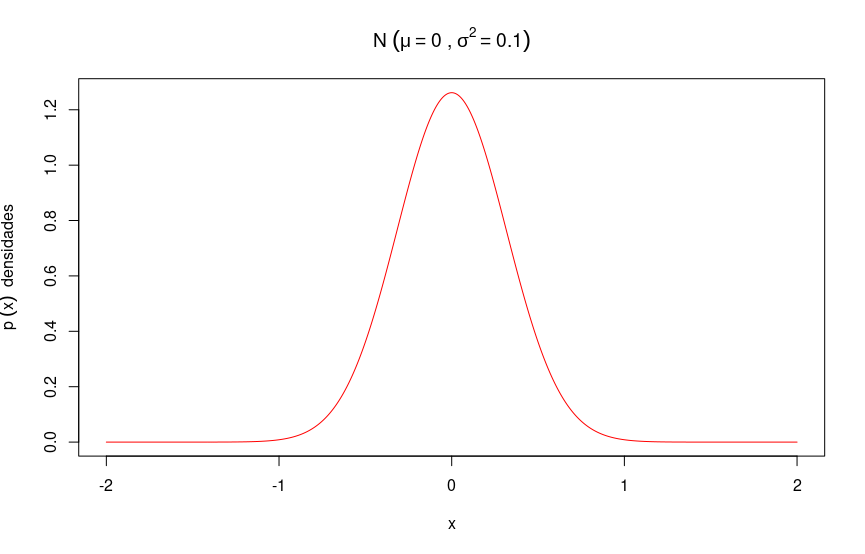
\includegraphics[width=0.48\textwidth]{img/N-m0-s01.png}
      }\hfill
      \subfloat[$\mu=1$ \label{fig:figura02}]{
        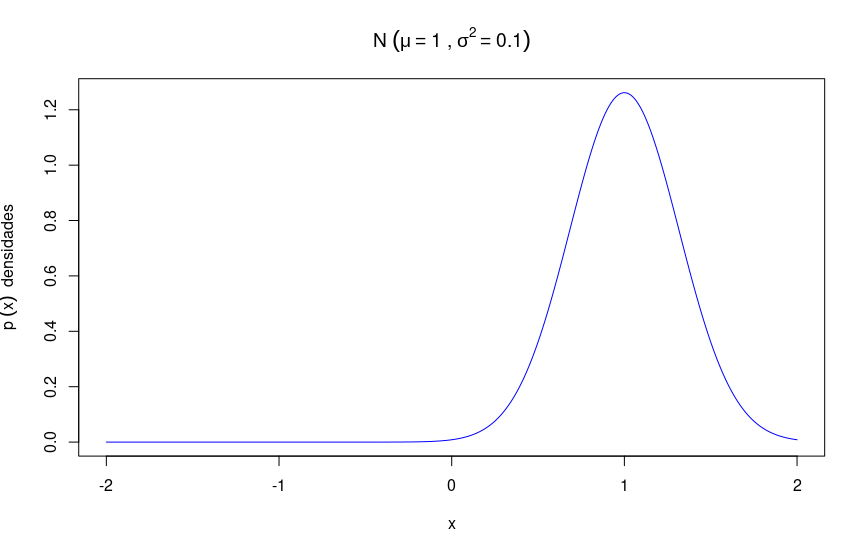
\includegraphics[width=0.48\textwidth]{img/N-mu1-s001.png}
      }        
      \caption{Distribuições gaussianas de mesma variância $\sigma^2=0,01$}
      \label{fig:gaussianas-1}       
    \end{figure}
    \begin{figure}[!htb]
      \centering
      \subfloat[$\mu=0$ \label{fig:figura03}]{
        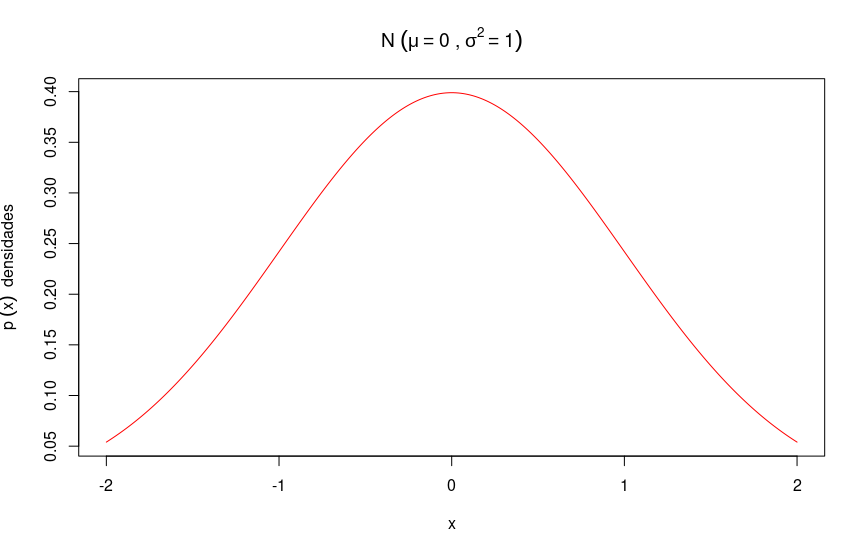
\includegraphics[width=0.48\textwidth]{img/fig-c.png}
      }\hfill
      \subfloat[$\mu=1$ \label{fig:figura04}]{
        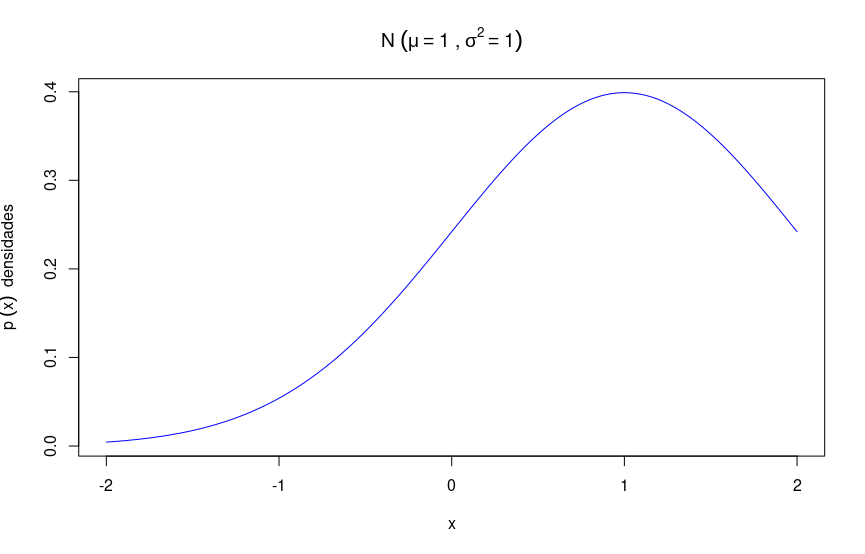
\includegraphics[width=0.48\textwidth]{img/fig-d.png}
      }        
      \caption{Distribuições gaussianas de mesma variância $\sigma^2=1$}
      \label{fig:gaussianas-2}       
    \end{figure}
    \begin{enumerate}[label=\alph *)]
      \item O gráfico da Figura\autoref{fig:figura02} assim como o gráfico da Figura\autoref{fig:figura04}, tem a sua forma deslocada para a direita, com relação aos gráficos da Figura\autoref{fig:figura01} e da Figura\autoref{fig:figura03} respectivamente, indicando que a curva é simétrica com relação a média $\mu$ e consequentemente, uma densidade de probabilidade maior em torno dessa média.
      \item Já os gráficos da \autoref{fig:gaussianas-1} diferem com relação aos gráficos da \autoref{fig:gaussianas-2}, pelo "achatamento" da curva, o que evidencia uma maior dispersão dos valores em torno da média. Quanto maior a variância $\sigma^2$, mais dispersos serão os valores da variável que se enquadra neste tipo de distribuição. 
    \end{enumerate}
  \end{sol}
\end{prob}  
% ---------------------------
    
% -----------------------------
% inserir o sumario
% -----------------------------------------------%
    \pdfbookmark[0]{\contentsname}{toc}
    \tableofcontents*
    \cleardoublepage
% -----------------------------------------------%
% ---------------
% INÍCIO DA LISTA
% ---------------
    \textual
    \pagestyle{cabecalholimpo}
% ---------------
% arquivos
    % ============| INÍCIO |===================
% --------------| Q01 |--------------------
\addcontentsline{toc}{section}{Problema 01}
\begin{prob}
Mostre que a expressão para o terceiro momento de uma distribuição binomial $\langle(\Delta N_1)^3 \rangle$ é $Npq(q-p)$
\begin{sol}
Partindo da definição \ref{def:n-momentum}
\begin{definition}[$n$-ésimo momento]
	\label{def:n-momentum}
	O momento de ordem $n$ em relação à média de uma variável aleatória $u$, é dado por:
	\begin{align}
		\label{eq:n-momentum}
		\langle(\Delta u)^n\rangle & =\langle\left(u-\langle u\rangle\right)^n\rangle
	\end{align}
\end{definition}
\noindent Deseja-se demostrar que $\langle\left(\Delta N_1\right)^3\rangle=Npq(q-p)$.
\begin{proof}
	\noindent Partindo da Definição: 0.0.1, tem-se que:
	\begin{align}
		\label{eq:3-momentum}
		\langle\left(\Delta N_1\right)^3\rangle & =\langle\left(N_1-\langle N_1\rangle\right)^3\rangle\nonumber \\
		\langle\left(\Delta N_1\right)^3\rangle & =\langle\left(N_1-\langle N_1\rangle\right)\left(N_1-\langle N_1\rangle\right)^2\rangle\nonumber \\
		\langle\left(\Delta N_1\right)^3\rangle & =\langle\left(N_1-\langle N_1\rangle\right)\left(N_1^2-2N_1\langle N_1\rangle+\langle N_1\rangle^2\right)\rangle\nonumber \\
		\langle\left(\Delta N_1\right)^3\rangle & =\langle N_1^3-3N_1^2\langle N_1\rangle+3N_1\langle N_1\rangle^2-\langle N_1\rangle^3\rangle\nonumber \\
		\langle\left(\Delta N_1\right)^3\rangle & =\langle N_1^3\rangle-3\langle N_1^2\rangle\langle \langle N_1\rangle\rangle+3\langle N_1\rangle\langle\langle N_1\rangle^2\rangle-\langle\langle N_1\rangle^3\rangle\nonumber \\
		\langle\left(\Delta N_1\right)^3\rangle & =\langle N_1^3\rangle-3\langle N_1^2\rangle\langle N_1\rangle+3\langle N_1\rangle\langle N_1\rangle^2-\langle N_1\rangle^3\nonumber \\
		\langle\left(\Delta N_1\right)^3\rangle & =\langle N_1^3\rangle-3\langle N_1^2\rangle\langle N_1\rangle+2\langle N_1\rangle^3
	\end{align}
	Agora, dado que
	\begin{align}
		\label{eq:N1}
		\langle N_1\rangle & =p\parder{}{p}\color{deepblue}{\underbrace{
			\color{black}{\sum_{N_1=0}^N\frac{N!}{N_1!N_2!}p^{N_1}p^{N_2}}
		}_{(p+q)^N}} \nonumber  \\
 		&=p\parder{}{p}\left(p+q\right)^N=pN\CancelTo[\color{deepred}]{p+q=1}{\left(p+q\right)^{N-1}}\nonumber \\
         & =Np
	\end{align}
	e
	\begin{align}
		\label{eq:N2}\langle N_1^2\rangle &=\left(p\parder{}{p}\right)\left\{\left(p\parder{}{p}\right)\left[\sum_{N_1=0}^N\frac{N!}{N_1!N_2!}p^{N_1}q^{N_2}\right]\right\}\nonumber \\
        &=\left(p\parder{}{p}\right)\left[pN\left(p+q\right)^{N-1}\right]\nonumber \\
        &=Np+Np^2\left(N-1\right)\CancelTo[\color{deepred}]{1}{\left(p+q\right)^{N-2}}\nonumber \\
        & =Np+Np^2\left(N-1\right)
	\end{align}
	analogamente tem-se
	\begin{align}
		\label{eq:N3}\langle N_1^3\rangle=\left(p\parder{}{p}\right)&\left(p\parder{}{p}\right)\left\{\left(p\parder{}{p}\right)\left[\sum_{N_1=0}^N\frac{N!}{N_1!N_2!}p^{N_1}q^{N_2}\right]\right\}\nonumber  \\
		=\left(p\parder{}{p}\right)&\left(p\parder{}{p}\right)\left[pN\left(p+q\right)^{N-1}\right]\nonumber \\
		=Np&\left\{\left(\parder{}{p}\right)\left[p\left(p+q\right)^{N-1}+p^2\left(N-1\right)\left(p+q\right)^{N-2}\right]\right\}\nonumber \\
		=Np&\left[\CancelTo[\color{deepred}]{1}{\left(p+q\right)^{N-1}}+p\left(N-1\right)\CancelTo[\color{deepred}]{1}{\left(p+q\right)^{N-2}}+2p\left(N-1\right)\CancelTo[\color{deepred}]{1}{\left(p+q\right)^{N-2}}+\right.\nonumber \\
        &\left.+p^2\left(N-1\right)\left(N-2\right)\CancelTo[\color{deepred}]{1}{\left(p+q\right)^{N-3}}\right]\nonumber \\
        &=Np\left[1+3p\left(N-1\right)+p^2\left(N-1\right)\left(N-2\right)\right]\nonumber \\
        &=Np\left\{1+p\left(N-1\right)\left[3+p\left(N-2\right)\right]\right\}
	\end{align}
	Utilizando os resultados das eqs. (\ref{eq:N1}), (\ref{eq:N2}) e (\ref{eq:N3}) na (\ref{eq:3-momentum}), temos que
	\begin{align}
		\langle\left(\Delta N_1\right)^3\rangle=Np&\left\{1+p\left(N-1\right)\left[3+p\left(N-2\right)\right]\right\}-\nonumber \\
       		   &-3Np\left[Np+Np^2\left(N-1\right)\right]+2N^3p^3\nonumber \\
		=Np&+Np^2\left(N-1\right)\left[3+p\left(N-2\right)\right]-\nonumber \\
       		   &-3N^2p^2-3N^2p^3\left(N-1\right)+2N^3p^3\nonumber \\
		=Np&+Np^2\left[3N-3+p\left(N-1\right)\left(N-2\right)\right]-\nonumber \\
			  -&3N^2p^2-3N^3p^3+3N^2p^3+2N^3p^3\nonumber \\
		=Np&\cancel{+3N^2p^2}-3Np^2+Np^3\left(N^2-3N+2\right)-\nonumber \\
               &\cancel{-3N^2p^2}-N^3p^3+3N^2p^3\nonumber \\
		=Np&-3Np^2\cancel{+N^3p^3}\cancel{-3N^2p^3}+2Np^3-\nonumber \\
               &\cancel{-N^3p^3}\cancel{+3N^2p^3}\nonumber \\
		=Np&-3Np^2+2Np^3\nonumber \\
		=Np&-2Np^2-Np^2+2Np^3\nonumber \\
		=Np&\left(1-2p\right)-Np^2\left(1-2p\right)\nonumber \\
		=Np&\left(1-2p\right)\CancelTo[\color{deepgreen}]{q}{\left(1-p\right)}\nonumber \\
		=Np&q\left(p+q-2p\right)\nonumber \\
		=Np&q\left(q-p\right)
	\end{align}
\end{proof}
\end{sol}
\end{prob}
% --------------| Q02 |--------------------
\newpage
\addcontentsline{toc}{section}{Problema 02}
\begin{prob}
	Uma variável aleatória $x$ está associada à densidade de probabilidade
	\begin{align}
		p(x) & =e^{-x},\qquad  \forall\; x\in \mathbb{R^\ast _+}\nonumber
	\end{align}
	\begin{enumerate}[label=\alph *)]
		\item Mostre que a densidade está normalizada a 1;
		\item Encontre o valor médio $\langle x\rangle$;
		\item Sendo $x_1$ e $x_2$ dois valores escolhidos de forma independente, encontre $\langle x_1+x_2\rangle$ e $\langle x_1x_2\rangle$.
	\end{enumerate}

	\begin{sol}
		\begin{enumerate}[label=\alph *)]
			\item Deseja-se demostrar que
			\begin{align}
				\int_{\mathbb{R^*_+}}p(x)dx & =\int_{\mathbb{R^*_+}}e^{-x}dx=1
			\end{align}
			\noindent Trata-se de uma integral imprópria em $\mathbb{R^*_+}$, portanto, façamos $a\to 0$ e $b\to +\infty$ de modo que tenhamos
			\begin{align}
				\int_{\mathbb{R^*_+}}p(x)dx & =\int_{a}^{b}e^{-x}dx=1
			\end{align}
			\begin{proof}
				\begin{align}
					\label{dem:a}
					\int_{\mathbb{R^*_+}}p(x)dx&=\int_{a}^{b}e^{-x}dx\nonumber \\
				    & =-e^{-x}\Biggr |_a^b\nonumber \\
				    &=e^{-a}-e^{-b}\nonumber \\
				    & =\CancelTo[\color{deepred}]{1}{\lim_{a\to 0}\left(\frac{1}{e^a}\right)}-\CancelTo[\color{deepgreen}]{0}{\lim_{b\to +\infty}\left(\frac{1}{e^b}\right)}\nonumber \\
				    & =1
				\end{align}
			\end{proof}
				\item Por definição definição
				\begin{definition}
					Se $x$ é uma variável aleatória contínua e $f(x)$ a sua função densidade de probabilidade, então:
					\begin{align}
						\label{def:valor-esperado-fdp}
						\langle x\rangle & =\int_{-\infty}^{+\infty}xf(x)dx
					\end{align}
				\end{definition}
				Avaliando primeiramente a integral num intervalo $[a,b]$ temos
				\begin{align}
					\int_{a}^{b}xe^{-x}dx & =-xe^{-x}\Biggr |_a^b+\int_{a}^{b}e^{-x}dx
					\label{eq:x-valor-esperado}
				\end{align}
				se $a\to 0$ e $b\to +\infty$, já vimos na Eq. (\ref{dem:a}) que a integral do lado direito converge e seu valor é 1, então
				\begin{align}
					\int_a^b xe^{-x}dx & =-xe^{-x}\Biggr |_a^{b}+1\nonumber\\
                  	& =1+\lim _{b\to +\infty}\left[(0)(1)-\frac{b}{e^{b}}\right]\nonumber\\
                  	& =1-\CancelTo[\color{deepred}]{0}{\lim _{b\to +\infty}\left(\frac{1}{be^b}\right)}\nonumber\\
                  	& =1
				\end{align}
				portanto
				\begin{align}
					\langle x\rangle & =1
				\end{align}
				\item Note que, dado o enunciado, podemos escrever $\langle x_1+x_2 \rangle=\langle x_1\rangle+\langle x_2\rangle$ e $\langle x_1x_2\rangle=\langle x_1\rangle\langle x_2\rangle$, além disso, da \autoref{eq:x-valor-esperado} sabemos  que $\langle x_1\rangle=1$ e $\langle x_2\rangle=1$, assim
				\begin{align}
					\langle x_2+x_1\rangle=&(1)+(1)=2\\
					\langle x_1\rangle\langle x_2\rangle=& (1)(1)=1
				\end{align}
		\end{enumerate}
	\end{sol}
\end{prob}
% --------------| Q03 |--------------------
\addcontentsline{toc}{section}{Problema 03}
\begin{prob}
	Obtenha o número de microestados acessíveis ao sistema de dois osciladores quânticos
	localizados e independentes, um com frequência fundamental $\omega_0$ e outro com $3\omega_0$, sendo a energia
	total do sistema $10\hbar \omega_0$. Explicite os números quânticos de cada oscilador que levam a esta
	energia total. \textbf{Sugestão: liste todas as possibilidades de números quânticos que levam ao resultado $E,N=10\hbar \omega_0$  (não são muitas!)}
	\begin{sol}
		Sabemos que
		\begin{align}
			E_n&=\left(n+\frac{1}{2}\right)\hbar\omega
		\end{align}
		Para os osciladores $n_1$ e $n_2$ teremos respectivamente
		\begin{align}
			E_{n_1}&=\left(n_1+\frac{1}{2}\right)\hbar\omega_0\\
			E_{n_2}&=\left(n_2+\frac{1}{2}\right)3\hbar\omega_0
		\end{align}
		sabemos também que $E_{1,2}=E_{n_1}+E_{n_2}$, decorre disto que
		\begin{align}
			\label{eq:osciladores-n1n2}
			\begin{split}
				E_{1,2}&=\left(n_1+\frac{1}{2}\right)\hbar\omega_0+\left(n_2+\frac{1}{2}\right)3\hbar\omega_0\\
				E_{1,2}&=n_1\hbar\omega_0+\frac{1}{2}\hbar\omega_0+3n_2\hbar\omega_0+\frac{3}{2}\hbar\omega_0\\
				E_{1,2}&=\left(n_1+3n_2\right)\hbar\omega_0+2\hbar\omega_0
			\end{split}
		\end{align}

		Sendo a energia total do sistema dos dois osciladores $E_{1,2}=10\hbar\omega_0$ então, resolvendo a \eqref{eq:osciladores-n1n2} para $n_2$ e arbitrando o valor de $n_1$ obtemos a tabela
\begin{table}[!ht]
	\centering
	\begin{tabular}{|c|c|c|c|c|c|c|c|c|}
	\hline
	\textbf{$n_1$} & \textbf{$n_1+3n_2=8$} & \textbf{$n_2$} & \textbf{$n_1$} & \textbf{$n_1+3n_2=8$} & \textbf{$n_2$} & \textbf{$n_1$} & \textbf{$n_1+3n_2=8$} & \textbf{$n_2$} \\ \hline
	0              & $0+3n_2=8$            & 8/3            & 3              & $3+3n_2=8$            & 5/3            & 6              & $6+3n_2=8$            & 2/3            \\ \hline
	1              & $1+3n_2=8$            & 7/3            & 4              & $4+3n_2=8$            & 4/3            & 7              & $7+3n_2=8$            & 1/3            \\ \hline
	2              & $2+3n_2=8$            & 2              & 5              & $5+3n_2=8$            & 1              & 8              & $8+3n_2=8$            & 0              \\ \hline
	\end{tabular}
	\caption{Combinações de números quânticos que levam ao valor de energia $E,N=10\hbar\omega_0$}
	\label{tab:numeros-quanticos}
\end{table}

Da tabela \ref{tab:numeros-quanticos}, encontramos 9 possibilidades que resultam na energia total do sistema $E_{1,2}=10\hbar\omega_0$, porém apenas 3 são realmente possíveis ($n_i=0,1,2,...$). Os únicos auto-estados possíveis ($n_1,n_2$) são portanto ($2,2$), (5,1) e (8,0).

Podemos obter o número de micro estados possíveis $\Omega(E,N,N)$ utilizando a relação
\begin{align}
	\label{eq:micro-estados}
	\Omega(E,N)&=\frac{(M+N-1)!}{M!(N-1)!}
\end{align}
Da equação \eqref{eq:osciladores-n1n2} tem-se que $M=n_1+3n_2$, se são 2 osciladores, então $N=2$, e uma vez que
\begin{align}
	E_{n_1,n_2}&=M\hbar\omega_0+\frac{N}{2}\hbar\omega_0
\end{align}
encontramos $M$ em termos da energia tal como segue
\begin{align}
	\begin{split}
		M\hbar\omega_0+2\hbar\omega_0&=E_{1,2}\\
		M\hbar\omega_0&=E_{1,2}-2\hbar\omega_0\\
		M&=\frac{E_{1,2}}{\hbar\omega_0}-2
	\end{split}
\end{align}
substituindo tudo em \eqref{eq:micro-estados}
\begin{align}
	\begin{split}
		\Omega(E,N)&=\frac{\Biggl[\left(\frac{E_{1,2}}{\hbar\omega_0}-2\right)+2-1\Biggr]!}{\left(\frac{E_{1,2}}{\hbar\omega_0}-2\right)!\left(2-1\right)!}\\
		\Omega(E,N)&=\frac{\left(\frac{E_{1,2}}{\hbar\omega_0}-1\right)!}{\left(\frac{E_{1,2}}{\hbar\omega_0}-2\right)!}\\
		\Omega(E,N)&=\frac{\left(\frac{10\hbar\omega_0}{\hbar\omega_0}-1\right)!}{\left(\frac{10\hbar\omega_0}{\hbar\omega_0}-2\right)!}\\
		\Omega(E,N)&=\frac{9!}{8!}\\
		\Omega(E,N)&=9
	\end{split}
\end{align}
Há um total de 9 estados mas somente 3 possíveis como havíamos observado.
	\end{sol}
\end{prob}

% --------------| Q04 |--------------------
\addcontentsline{toc}{section}{Problema 04}
\begin{prob}
	Em um modelo simplificado para um gás de partículas, o volume do sistema é dividido em
	 $V$ células de volume unitário (pode ser tratado como um “número” de volumes). Encontre o 
	 número	de maneiras de distribuir:
	 \begin{enumerate}[label=\alph *)]
	 	\item $N$ partículas distinguíveis $(0\leq N\leq V)$ entre $V$ células de modo que cada célula
	 	possa estar vazia ou ocupada por uma única partícula.
	 	\item Como a resposta é alterada se as partículas forem indistinguíveis?
	 	\item \textbf{Referente ao item b:} considere que $V$ e $N$ sejam muito grandes e defina a variável $v=V/N$.
	 	Utilize a fórmula de Stirling e mostre que
	 	\begin{align}
	 		\frac{1}{N}\ln \Omega&=v\ln v - (v-1)\ln (v-1)
	 	\end{align}
	 \end{enumerate}
\end{prob}

\begin{sol}
	\begin{enumerate}[label=\alph *)]
		\item Dado $N$ o número de partículas distintas do gás, deseja-se arranjá-las em $V$ volumes tal que $V\geq N$.
		
		\par\noindent\emph{modelização:}

		Imaginemos primeiramente 4 partículas $N_j$ distintas, para 7 volumes $V_k$

		\begin{table}[!ht]
			\centering
			\begin{tabular}{|l|l|l|l|l|l|l|}
			\hline
			$V_1$ & $V_2$ & $V_3$ & $V_4$ & $V_5$ & $V_6$ & $V_7$ \\ \hline
			$N_1$ & $N_2$ &       &       & $N_3$ &       & $N_4$ \\ \hline
			\end{tabular}
		\end{table}
		Sendo partículas distinguíveis, a permutação $N_1\longleftrightarrow N_2$ gera um novo arranjo diferente

		\begin{table}[!ht]
			\centering
			\begin{tabular}{|l|l|l|l|l|l|l|}
			\hline
			$V_1$ & $V_2$ & $V_3$ & $V_4$ & $V_5$ & $V_6$ & $V_7$ \\ \hline
			$N_2$ & $N_1$ &       &       & $N_3$ &       & $N_4$ \\ \hline
			\end{tabular}
		\end{table}
		Neste caso, o número de arranjos distintos é dado pela permutação simples de 7 volumes tomados a cada 4 partículas, ou seja $_7P_4$
		\begin{align}
			_7P_4&=\frac{7!}{(7-4)!}=840
		\end{align}
		Logo, para $V$ volumes e $N$ partículas, temos simplesmente
		\begin{align}
			_VP_N&=\frac{V!}{(V-N)!}
		\end{align}
		portanto,
		\begin{align}
			\Omega (V,N)&=\frac{V!}{(V-N)!}
		\end{align}
			\item Caso as partículas sejam indistinguíveis, então as permutações $N\longleftrightarrow N$ não mais geram novos arranjos, como podemos perceber a seguir
			
			\begin{table}[!ht]
				\centering
				\begin{tabular}{|l|l|l|l|l|l|l|}
				\hline
				$V_1$ & $V_2$ & $V_3$ & $V_4$ & $V_5$ & $V_6$ & $V_7$ \\ \hline
				$N$   & $N$   &       &       & $N$   &       & $N$   \\ \hline
				\end{tabular}
			\end{table}
			e o número de arranjos possíveis, para o caso dos 7 volumes e 4 partículas é dado pela combinação $7\choose 4$, isto é
			\begin{align}
				7C_4&={7\choose 4}=\frac{7!}{(7-4)!4!}=35
			\end{align}
			um número bem menor de arranjos! Generalizando para $V$ volumes e $N$ partículas indistinguíveis teremos
			\begin{align}
				\label{eq:N-indist}
				\Omega (V,N)&=\frac{V!}{(V-N)!N!}
			\end{align}
			\item Pela fórmula de \emph{stirling} tem-se que
			\begin{align}
				\ln \N!&=N\ln N -N+O(\ln N)
			\end{align}
			aplicando o logaritmo natural em ambos os lados da \eqref{eq:N-indist}, obtêm-se
			\begin{align}
				\begin{split}
					\label{eq:aprox-stirling0}
					\ln \Omega&=\ln\left[\frac{V!}{(V-N!)N!}\right]\\
					&=\ln V!-\biggl[\ln\left(V-N\right)!+\ln N!\biggr]	
				\end{split}				
			\end{align}
			usando a série assintótica de stirling em \eqref{eq:aprox-stirling0}	
			\begin{equation}
				\label{eq:aprox-stirling1}
				\begin{split}
					\ln \Omega(V,N)=V\ln V&-\cancel{V}-\Bigl[\left(V-N\right)\ln\left(V-N\right)-\left(\cancel{V}-\cancel{N}\right)+\\
					&+N\ln N-\cancel{N}\Bigr]+O\left(\ln V\right)+O\left[\ln (V-N)\right]+\\
					&+O\ln\left(N\right)
				\end{split}
			\end{equation}
			Tomando $N$ e $V$ suficientemente grandes, podemos descartar os termos da ordem de $\ln$ da série de stirling, ficando apenas com os primeiros termos, além disso, usando $v=V/N$ na \eqref{eq:aprox-stirling1} ficamos com
			\begin{proof}
				\begin{align}
					\begin{split}
						\ln\Omega(v,N)=vN\ln vN&-\Bigl[\left(vN-N\right)\ln\left(vN-N\right)+N\ln N\Bigr]\\
						=vN\ln v+&vN\ln N-\Bigl\{N\left(v-1\right)\ln \Bigl[N\left(v-1\right)\Bigr]+N\ln N\Bigr\}\\
						=N\Bigl\{v\ln v&+\cancel{v\ln N}-\Bigl[\cancel{\left(v-1\right)\ln N}+\left(v-1\right)\ln (v-1)\Bigr]+\cancel{\ln N}\Bigr\}\\
						=N\Bigl[v\ln v&-\left(v-1\right)\ln\left(v-1\right)\Bigr]		
					\end{split}
				\end{align}
				e por fim, dividindo-se ambos os lados da igualdade por $N$, chegamos em
				\begin{align}
						\frac{1}{N}\ln\Omega(v,N)=v\ln v-&\left(v-1\right)\ln\left(v-1\right)
				\end{align}
			\end{proof}
	\end{enumerate}
	
\end{sol}
% --------------| Q05 |--------------------
\addcontentsline{toc}{section}{Problema 05}
\begin{prob}
	A partir da equação de van der Waals
	\begin{align}
		p&=\frac{RT}{v-b}-\frac{a}{v^2}
	\end{align}
	e sabendo que
	\begin{align}
		\label{eq:calor-especifico-vcte}
		c_V&=T\left(\parder{s}{T}\right)_v=c
	\end{align}
	Obtenha a relação fundamental na representação de Helmholtz $f(T,v)$. Logo após, mostre que a densidade de energia é dada por
	\begin{align}
		u&=cT-\frac{a}{v}
	\end{align}
	\begin{sol}
		Partindo da relação
		\begin{align}
			\label{eq:5.1}
			F&=U-TS
		\end{align}
		tem-se que
		\begin{align}
			\label{eq:5.2}
			\begin{split}
				dF&=dU-d(TS)\\
				dF&=dU-TdS-SdT
			\end{split}
		\end{align}
		Escrevendo a 1ª Lei da termodinâmica para o problema
		\begin{align}			
			dU&=TdS-pdV
			\label{eq:1-lei-termodinamica}
		\end{align}
		e utilizando na \eqref{eq:5.2}
		\begin{align}
			\begin{split}
				df&=\color{deepgreen}{\underbrace{\color{black}{(TdS-PdV)}}_{dU}}\color{black}{-TdS-SdT}\\
				dF&=-SdT-pdV
				\label{eq:5.3}
			\end{split}
		\end{align}
		fazendo $s=S/N$ e $v=V/N$
		\begin{align}
			df(T,v)=-sdT-pdv
			\label{eq:5.4}
		\end{align}
		De modo geral, uma diferencial exata pode sempre ser escrita da seguinte forma
		\begin{align}
			\label{eq:5.41}
			df(T,v)&=\left(\parder{f}{T}\right)_vdT+\left(\parder{f}{v}\right)_Tdv
		\end{align}
		resulta da \eqref{eq:5.4} e da \eqref{eq:5.41} que
		\begin{subequations}
			\begin{align}					
					\left(\parder{f}{T}\right)_v&=-s\label{eq:5.5a}\\
					\left(\parder{f}{v}\right)_T&=-p\label{eq:5.5b}
			\end{align}
		\end{subequations}
		reescrevendo a \eqref{eq:5.4} em termos das variáveis do problema
		\begin{align}
			\label{eq:5.6}
			df(T,v)=-sdT+\left(\frac{a}{v^2}-\frac{RT}{v-b}\right)dv
		\end{align}
		Precisamos construir a função $s=s(T,v)$. Assumindo que estas funções possuam também segundas derivadas definidas, a condição de diferenciabilidade exige que
		\begin{align}
			\left[\parder{}{v}\left(\parder{f}{T}\right)_v\right]_T&=\left[\parder{}{T}\left(\parder{f}{v}\right)_T\right]_v
		\end{align}
		essa condição aplicada as \eqref{eq:5.5a} e \eqref{eq:5.5b}, reduz a
		\begin{subequations}
			\begin{align}
				\left[\parder{}{v}\left(\parder{f}{T}\right)_v\right]_T&=-\left(\parder{s}{v}\right)_T \label{eq:cond-diferenciabilidde-s}\\			
				\left[\parder{}{T}\left(\parder{f}{v}\right)_T\right]_v&=-\left(\parder{p}{T}\right)_v \label{eq:cond-diferenciabilidde-p}
			\end{align}
		\end{subequations}
		observe que $s=s(T,v)$, é
		\begin{align}
			\label{eq:derivada-funcao-s}
			ds(T,v)&=\left(\parder{s}{v}\right)_Tdv+\left(\parder{s}{T}\right)_vdT
		\end{align}
		Achar a $(\partial_vs)_T$, é simples, basta utilizar a condição de diferenciabilidade expressa pelas relações \eqref{eq:cond-diferenciabilidde-s} e \eqref{eq:cond-diferenciabilidde-p}, de modo que
		\begin{align}
			\left(\parder{s}{v}\right)_T&=\left(\parder{p}{T}\right)_v
		\end{align} 
		i.e.:
		\begin{align}
			\begin{split}
				\label{eq:s-funcao-v}
				\left(\parder{s}{v}\right)_T&=\left[\parder{}{T}\left(\frac{RT}{v-b}-\frac{a}{v^2}\right)\right]\\
				\left(\parder{s}{v}\right)_T&=\frac{R}{v-b}
			\end{split}
		\end{align}
		agora, a relação $(\partial_Ts)_v$ é dada pelo problema [vide eq.:\eqref{eq:calor-especifico-vcte}], atualizando a \eqref{eq:derivada-funcao-s} tem se
		\begin{align}
			ds(T,v)&=\left(\frac{R}{v-b}\right)dv+\frac{c_v}{T}dT
		\end{align}
		cujo a solução é conhecida, pelo o que segue
		\begin{align}
			\begin{split}
				s(v,T)&=\int_{v}\left(\frac{R}{v-b}\right)dv+g(T)\\
				s(v,T)&=R\ln(v-b)+g(T)\\
				\left(\parder{s}{T}\right)_T&=\frac{dg(T)}{dT}=\frac{c_v}{T}\implies g(T)=c_v\ln T								
			\end{split}
		\end{align}
		\begin{align}
			\boxed{
					s(v,T)=R\ln (v-b)+c_v\ln T
				}
		\end{align}
		procedendo de forma semelhante com a \eqref{eq:5.6} obtemos
		\begin{align}
			\begin{split}
				f(v,T)&=-\left[R\ln (v-b)+c_v\ln T\right]dT+\left(\frac{a}{v^2}-\frac{RT}{v-b}\right)dv\\
				f(v,T)&=-\int_T\left[R\ln(v-b)+c_v\ln T\right]dT+h(v)\\
				f(v,T)&=-RT\ln(v-b)-c_vT(\ln T-1)+h(v)\\
				\left(\parder{f}{v}\right)_T&=-\frac{RT}{v-b}+\frac{dh(v)}{dv}=\frac{a}{v^2}-\frac{RT}{v-b}\implies h(v)=-\frac{a}{v}
			\end{split}			
		\end{align}
		a relação fundamental da equação de van der Waals na representação de Helmholtz $f(T,v)$, fica
		\begin{align}
			\boxed{
				f(v,T)=-RT\ln(v-b)-c_vT(\ln T-1)-\frac{a}{v}
			}
		\end{align}
		Tendo encontrado $f$ e $s$, obtêm-se a representação em termos da densidade de energia bastando fazer
		\begin{align}
			u&=f+Ts
		\end{align}
		na \eqref{eq:5.1}, logo
		\begin{align}
			\begin{split}
				u&=-RT\ln(v-b)-c_vT(\ln T-1)-\frac{a}{v}+T\left[R\ln (v-b)+c_v\ln T\right]\\
				u&=\cancel{-RT\ln(v-b)}\cancel{-c_vT\ln T}+c_vT-\frac{a}{v}\cancel{+TR\ln (v-b)}\cancel{+Tc_v\ln T}
			\end{split}
		\end{align}
		\begin{align}
			\boxed{
				u=c_v-\frac{a}{v}
			}
		\end{align}
	\end{sol}
\end{prob}
% --------------| Q06 |--------------------
\addcontentsline{toc}{section}{Problema 06}
\begin{prob}
	Considere um fluido puro de uma componente. Utilize as relações de Maxwell na representação
de Helmholtz para mostrar que
\begin{align}
	\label{eq:relacao-prob6.1}
	\left(\parder{s}{v}\right)_T&=\left(\parder{p}{T}\right)_v
\end{align}
Com este resultado, mostre que
\begin{align}
	\label{eq:relacao-prob6.2}
	\left(\parder{c_v}{v}\right)_T&=T\left(\parder{^2p}{T^2}\right)_v
\end{align}
\begin{sol}
	Considere a representação de Helmholtz na forma diferencial
	\begin{align}
		\label{eq:representacao-helmholtz}
		dF&=-SdT-pdV+\mu dN
	\end{align}
	As relações de Maxwell na representação de Helmholtz, decorrem da condição de existência da função $F(T,V,N)$ e de suas derivadas, como já visto no problema anterior, uma vez que podemos escrever
	\begin{align}
		\label{eq:representacao-helholtz-delparc}
		dF(T,V,N)&=\left(\parder{F}{T}\right)_{V,N}dT+\left(\parder{F}{V}\right)_{T,N}dV+\left(\parder{F}{N}\right)_{T,V}dN
	\end{align}
	a condição de existência das derivadas primeiras e segundas, necessita que
	\begin{subequations}
		\begin{align}
			\left[\parder{}{V}\left(\parder{F}{T}\right)_{V,N}\right]_{T,N}=\left[\parder{}{T}\left(\parder{F}{V}\right)_{T,N}\right]_{V,N}\label{eq:d2fdvdt=d2fdtdv}\\
			\left[\parder{}{N}\left(\parder{F}{T}\right)_{V,N}\right]_{T,V}=\left[\parder{}{T}\left(\parder{F}{N}\right)_{T,V}\right]_{V,N}\label{eq:d2fdndt=d2fdtdn}\\
			\left[\parder{}{N}\left(\parder{F}{V}\right)_{T,N}\right]_{T,V}=\left[\parder{}{V}\left(\parder{F}{N}\right)_{T,V}\right]_{T,N}\label{eq:d2fdndv=d2fdvdn}
		\end{align}
	\end{subequations}
	o que combinado com as expressões \eqref{eq:representacao-helmholtz} e \eqref{eq:representacao-helholtz-delparc} resulta diretamente nas relações de Maxwell	
	\begin{subequations}
		\begin{align}
			-\left[\parder{S}{V}\right]_{T,N}&=-\left[\parder{p}{T}\right]_{V,N}\label{eq:maxwell-helmholtz-ps}\\
			-\left[\parder{S}{N}\right]_{T,V}&=\left[\parder{\mu}{T}\right]_{V,N}\label{eq:maxwell-helmholtz-sm}\\
			-\left[\parder{p}{N}\right]_{T,V}&=\left[\parder{\mu}{V}\right]_{T,N}\label{eq:maxwell-helmholtz-pm}
		\end{align}
	\end{subequations}
	Assim, a relação \eqref{eq:relacao-prob6.1} fica justificada pelas relações \eqref{eq:d2fdvdt=d2fdtdv} e \eqref{eq:maxwell-helmholtz-ps}, quando tomadas sobre as densidades $v=V/N$ e $s=S/N$
	\begin{align}
		\left(\parder{s}{v}\right)_{T}&=\left(\parder{p}{T}\right)_{v}
	\end{align}
	tomando a $\partial_T$ em ambos os lados da igualdade acima, tem-se
	\begin{align}
		\left[\parder{}{T}\left(\parder{s}{v}\right)_T\right]_{v}=\left[\parder{}{T}\left(\parder{p}{T}\right)_v\right]_v
	\end{align}
	ou, equivalentemente
	\begin{align}
		\left[\parder{}{v}\left(\parder{s}{T}\right)_v\right]_T=\left(\parder{^2p}{T^2}\right)_v
	\end{align}
	mas $T(\partial_Ts)_v=c_v$, então, multiplicando ambos lados da igualdade acima por $T$ tem-se o que deseja-se demonstrar
	\begin{align}
		\begin{split}
			\left[\parder{}{v}T\left(\parder{s}{T}\right)_v\right]_T&=T\left(\parder{^2p}{T^2}\right)_v\\
			\left(\parder{c_v}{v}\right)&=T\left(\parder{^2p}{T^2}\right)_v\
		\end{split}
	\end{align}
\end{sol}
\end{prob}

% --------------| Q07 |--------------------
\addcontentsline{toc}{section}{Problema 07}
\begin{prob}
	Para o problema do paramagneto de spin $1/2$, partindo da entropia obtida em aula, mostre que:
	\begin{enumerate}[label=\alph *)]
		\item
		\begin{align}
			\frac{1}{T}&=\frac{k_B}{2\mu_0H}\Biggl[\ln\left(1-\frac{u}{\mu_0H}\right)-\ln\left(1+\frac{u}{\mu_0H}\right)\Biggr]			
		\end{align}
		\item
		\begin{align}
			u&=-\mu_0H\tanh\left(\frac{\mu_0H}{k_BT}\right)			
		\end{align}
		\item Utilizando a relação entre densidade de energia e magnetização, obtenha a suscetibilidade
		magnética
		\begin{align}
			\chi(T,H)&=\left(\parder{m}{H}\right)_T=\frac{\mu_0^2}{k_BT}\cosh^{-2}\frac{\mu_0H}{k_BT}
		\end{align}
	\end{enumerate}
	\begin{sol}Em sala de aula, obtemos para a densidade de entropia a seguinte expressão
		\begin{align}
			s(u)&=k_B\ln 2-\frac{k_B}{2}\left(1-\frac{u}{\mu_0H}\right)\ln\left(1-\frac{u}{\mu_0H}\right)-\frac{k_B}{2}\left(1+\frac{u}{\mu_0H}\right)\ln\left(1+\frac{u}{\mu_0H}\right)
		\end{align}
		\begin{enumerate}[label=\alph *)]
			\item Basta avaliarmos $\partial_u s(u)$, sendo assim
			\begin{proof}[Demostração 7(a)]
				\begin{align}
					\label{eq:7A}
					\begin{split}
						\frac{1}{T} = \parder{s(u)}{u}=-\frac{k_B}{2} \Bigg[ \Bigg. & 
						-\left(\frac{1}{\mu_0H}\right)\ln\left(1-\frac{u}{\mu_0H}\right) + \\
						& + \CancelTo[\color{deepgreen}]{1}{\left(1-\frac{u}{\mu_0H}\right)\left(1-\frac{u}{\mu_0H}\right)^{-1}}\left(-\frac{1}{\mu_0H}\right) + \\
						& +\CancelTo[\color{deepgreen}]{1}{\left(1+\frac{u}{\mu_0H}\right)\left(1+\frac{u}{\mu_0H}\right)^{-1}} \left(\frac{1}{\mu_0H}\right) + \\
						& + \left(\frac{1}{\mu_0H}\right)\ln\left(1+\frac{u}{\mu_0H}\right)
						\Bigg. \Bigg]\\
						\frac{1}{T}=\frac{k_B}{2\mu_0H}\Bigg[&\ln\left(1-\frac{u}{\mu_0H}\right)-\ln\left(1+\frac{u}{\mu_0H}\right)\cancel{+1-1} \Bigg]\\
						\frac{1}{T}=\frac{k_B}{2\mu_0H}\Bigg[&\ln\left(\frac{\mu_0H-u}{\mu_0H+u}\right)\Bigg]
					\end{split}
				\end{align}
			\end{proof}
			\item Agora basta invertermos a \eqref{eq:7A}, rearranjando os termos
			\begin{align}				
				\begin{split}
						\frac{1}{T}&=\frac{k_B}{2\mu_0H}\left[\ln\left(\frac{\mu_0H-u}{\mu_0H+u}\right)\right]\\
						\frac{2\mu_0H}{k_BT}&=\ln\left(\frac{\mu_0H-u}{\mu_0H+u}\right)
				\end{split}
			\end{align}
			ou
			\begin{align}				
				\beta&=\frac{1}{k_BT} & \alpha&=\mu_0H				
			\end{align}
			\begin{align}
				\label{eq:7B0}
				2\beta\alpha&=\ln\left(\frac{\alpha-u}{\alpha+u}\right)
			\end{align}
			\begin{proof}[Demostração 7(b)]
				Aplicando a inversa do logaritmo natural em \eqref{eq:7B0} 
				\begin{align}
					\label{eq:7B}
					\begin{split}
						e^{2\alpha\beta}&=\frac{\alpha-u}{\alpha+u}\\
						e^{2\alpha\beta}\left(\alpha+u\right)&=\alpha-u\\
						\alpha e^{2\alpha\beta}+ue^{2\alpha\beta}&=\alpha-u\\
						ue^{2\alpha\beta}+u&=\alpha-\alpha e^{2\alpha\beta}\\
						u\left(e^{2\alpha\beta}+1\right)&=\alpha\left(1-e^{2\alpha\beta}\right)\\
						u&=\alpha\left(\frac{1-e^{2\alpha\beta}}{1+e^{2\alpha\beta}}\right)\left(\frac{-e^{-\alpha\beta}}{-e^{-\alpha\beta}}\right)\\
						u&=-\alpha\left[\frac{-e^{-\alpha\beta}\left(1-e^{2\alpha\beta}\right)}{e^{-\alpha\beta}\left(1+e^{2\alpha\beta}\right)}\right]\\
						u&=-\alpha\left(\frac{e^{-\alpha\beta}-e^{\alpha\beta}}{e^{-\alpha\beta}+e^{\alpha\beta}}\right)\\
						u&=-\alpha\tanh(\alpha\beta)\\
						u&=-\mu_0H\tanh\left(\frac{\mu_0H}{k_BT}\right)
					\end{split}
				\end{align}
			\end{proof}
			\item Considerando que
			\begin{align}
				\begin{split}
					m&=-\frac{u}{H}\\
					m&=\mu_0\tanh\left(\frac{\mu_0H}{k_BT}\right)
				\end{split}
			\end{align}
			e utilizado $d/dx\tanh(x)=\cosh^{-2}(x)$. Basta avaliarmos $\partial_Hm$, como segue
			\begin{align}
				\begin{split}					
				\chi(T,H)&=\left(\parder{m}{H}\right)_T\\
				\chi(T,H)&=\parder{}{H}\left[\mu_0\tanh\left(\frac{\mu_0H}{k_BT}\right)\right]\\
				\chi(T,H)&=\mu_0\left[\cosh^{-2}\left(\frac{\mu_0H}{k_BT}\right)\right]\left(\frac{\mu_0}{k_BT}\right)\\
				\chi(T,H)&=\frac{\mu_0^2}{k_BT}\cosh^{-2}\left(\frac{\mu_0H}{k_BT}\right)
				\end{split}
			\end{align}
		\end{enumerate}
	\end{sol}
\end{prob}

% --------------| Q08 |--------------------
\addcontentsline{toc}{section}{Problema 08}
\begin{prob}
	Partindo da expressão para o número de microestados acessíveis do sólido de Einstein
	\begin{align}
		\Omega(E,N)&=\frac{\left(\frac{E}{\hbar\omega}+\frac{N}{2}-1\right)!}{\left(\frac{E}{\hbar\omega}-\frac{N}{2}\right)!\left(N-1\right)!}
	\end{align}
	obtenha a densidade de entropia do sólido de Einstein.
	\begin{sol}
		Dado a densidade de entropia, como
		\begin{align}
			\label{eq:post-entropia}
			s(u)&=\displaystyle \lim_{N \to \infty;\frac{E}{N}=u}\frac{1}{N}k_B\ln\Omega(E,N)
		\end{align}
		Vamos primeiro aplicar o logaritmo ao número de microestados acessíveis $\Omega(E,N)$
		\begin{align}
			\label{eq:dens-entropia-sol-einstein}
			\begin{split}
				\ln\Omega(E,N)&=\ln\Biggl[\frac{\left(\frac{E}{\hbar\omega}+\frac{N}{2}-1\right)!}{\left(\frac{E}{\hbar\omega}-\frac{N}{2}\right)!\left(N-1\right)!}\Biggr]\\
				&=\ln\left(\frac{E}{\hbar\omega}+\frac{N}{2}-1\right)!-\biggl[\ln\left(\frac{E}{\hbar\omega}-\frac{N}{2}\right)!+\ln\left(N-1\right)\biggr]!
			\end{split}
		\end{align}
		Usando a expansão de stirling em \eqref{eq:dens-entropia-sol-einstein}
		\begin{align}
			\begin{split}
				\ln\Omega(E,N)=&\left(\frac{E}{\hbar\omega}+\frac{N}{2}-1\right)\ln\left(\frac{E}{\hbar\omega}+\frac{N}{2}-1\right)-\left(\frac{E}{\hbar\omega}+\frac{N}{2}-1\right)+\\
				&\qquad-\Biggl[\left(\frac{E}{\hbar\omega}-\frac{N}{2}\right)\ln\left(\frac{E}{\hbar\omega}-\frac{N}{2}\right)-\left(\frac{E}{\hbar\omega}-\frac{N}{2}\right)+\\&\qquad\qquad+\left(N-1\right)\ln\left(N-1\right)-\left(N-1\right)\Biggr]\\
				\ln\Omega(E,N)=&\left(\frac{E}{\hbar\omega}+\frac{N}{2}-1\right)\ln\left[N\left(\frac{E}{N\hbar\omega}+\frac{1}{2}-\frac{1}{N}\right)\right]-\left(\frac{E}{\hbar\omega}-\frac{N}{2}\right)\times\\&\quad\times\ln\left[N\left(\frac{E}{N\hbar\omega}-\frac{1}{2}\right)\right]-(N-1)\ln\left[N\left(1-\frac{1}{N}\right)\right]-\cancel{\left(\frac{E}{\hbar\omega}+{\frac{N}{2}}-{1}\right)}+\\
				&\qquad+\cancel{\left(\frac{E}{\hbar\omega}-\frac{N}{2}\right)+(N-1)}\\
				\ln\Omega(E,N)=&\left(\frac{E}{\omega\hbar}+\frac{N}{2}-1\right)\left[\ln N+\ln\left(\frac{E}{N\hbar\omega}+\frac{1}{2}-\frac{1}{N}\right)\right]-\left(\frac{E}{\hbar\omega}-\frac{N}{2}\right)\times\\&\quad\times\left[\ln N+\ln\left(\frac{E}{N\omega\hbar}-\frac{1}{2}\right)\right]-(N-1)\left[\ln N+\ln\left(1-\frac{1}{N}\right)\right]\\
				\ln\Omega(E,N)=&\left(\frac{E}{\omega\hbar}+\frac{N}{2}-1\right)\ln\left(\frac{E}{N\omega\hbar}+\frac{1}{2}-\frac{1}{N}\right)-\left(\frac{E}{\hbar\omega}-\frac{N}{2}\right)\ln\left(\frac{E}{N\omega\hbar}-\frac{1}{2}\right)+\\&\quad-(N-1)\ln\left(1-\frac{1}{N}\right)+\cancel{\left(\frac{E}{\omega\hbar}+\frac{N}{2}-1\right)\ln N}-\cancel{\left(\frac{E}{\hbar\omega}-\frac{N}{2}\right)\ln N}+\\&\qquad-\cancel{(N-1)\ln N}
			\end{split}
			\label{eq:ln-Omega}
		\end{align}
		dividindo \eqref{eq:ln-Omega} por $N$ obtêm-se
		\begin{align}
			\label{eq:omega-div-n}
			\begin{split}
				\frac{1}{N}\ln\Omega(E,N)=&\left(\frac{E}{N\hbar\omega}+\frac{1}{2}-\frac{1}{N}\right)\ln\left(\frac{E}{N\hbar\omega}+\frac{1}{2}-\frac{1}{N}\right)-\left(\frac{E}{N\hbar\omega}-\frac{1}{2}\right)\times\\&\quad\times\ln\left(\frac{E}{N\hbar\omega}-\frac{1}{2}\right)-\left(1-\frac{1}{N}\right)\ln\left(1-\frac{1}{N}\right)
			\end{split}
		\end{align}
		multiplicando por $k_B$ e aplicando o limite termodinâmico em \eqref{eq:omega-div-n} tem-se
		\begin{align}
			\label{eq:lim-ln-Omega}
			\begin{split}
				\displaystyle \lim_{N \to \infty;\frac{E}{N}=u}\frac{1}{N}k_B\ln\Omega(E,N)&=k_B\left(\CancelTo[\color{deepgreen}]{u}{\frac{E}{N}}\frac{1}{\hbar\omega}+\frac{1}{2}-\CancelTo[\color{deepred}]{0}{\frac{1}{N}}\right)\ln\left(\CancelTo[\color{deepgreen}]{u}{\frac{E}{N}}\frac{1}{\hbar\omega}+\frac{1}{2}-\CancelTo[\color{deepred}]{0}{\frac{1}{N}}\right)+\\
				&\quad-k_B\left(\CancelTo[\color{deepgreen}]{u}{\frac{E}{N}}\frac{1}{\hbar\omega}-\frac{1}{2}\right)\ln\left(\CancelTo[\color{deepgreen}]{u}{\frac{E}{N}}\frac{1}{\hbar\omega}-\frac{1}{2}\right)-k_B(1-\CancelTo[\color{deepred}]{0}{\frac{1}{N}})\ln(1-\CancelTo[\color{deepred}]{0}{\frac{1}{N}})\\\therefore \\
				s(u)&=k_B\left(\frac{u}{\hbar\omega}+\frac{1}{2}\right)\ln\left(\frac{u}{\hbar\omega}+\frac{1}{2}\right)-k_B\left(\frac{u}{\hbar\omega}-\frac{1}{2}\right)\ln\left(\frac{u}{\hbar\omega}-\frac{1}{2}\right)
			\end{split}
		\end{align}
	\end{sol}
\end{prob}

% --------------| Q09 |--------------------
\addcontentsline{toc}{section}{Problema 09}
\begin{prob}
	A distribuição de velocidades de Maxwell – Boltzmann, para um problemas onde nenhuma
	direção seja favorecida, pode ser escrita como
	\begin{align}
		p(\mathbf{v})d^3\mathbf{v}&=\left(\frac{2\pi k_BT}{m}\right)^{-\frac{3}{2}}e^{-\left(\frac{m\mathbf{v^2}}{2k_BT}\right)}4\pi v^2dv
	\end{align}
	logo, temos a distribuição dependente do módulo das velocidades:
	\begin{align}
		p(v)&=4\pi\left(\frac{2\pi k_BT}{m}\right)^{-\frac{3}{2}}v^2e^{-\left(\frac{mv^2}{2k_BT}\right)}
	\end{align}
	Mostre que:
	\begin{enumerate}[label=\alph *)]
		\item o valor de velocidade para o qual a distribuição é máxima vale $v_{max}=\sqrt{\frac{2k_BT}{m}}$
		\item $\langle v\rangle=\sqrt{\frac{8k_BT}{\pi m}}$
		\item $\langle v^2\rangle=\frac{3k_BT}{m}$
		\item A energia cinética média $\langle K\rangle=\left\langle \frac{1}{2}mv^2\right\rangle=\frac{3}{2}k_BT$
	\end{enumerate}
	Pode utilizar tabelas e programas para as integrais! Apenas deixe claro a fórmula que está utilizando
	para resolver cada caso.
	\begin{sol}
		\begin{enumerate}[label=\alph *)]
			\item A função distribuição de probabilidade é máxima, quando
			\begin{align}
				\parder{p(v)}{v}\Biggr |_{v=v_{\textrm{máx}}}&=0
			\end{align}
			Tomando a derivada de $p(v)$ com relação à variável $v$
			\begin{align}
				\begin{split}
					\parder{p(v)}{v}&=\parder{}{v}\left[4\pi\left(\frac{2\pi k_BT}{m}\right)^{-\frac{3}{2}}v^2e^{-\left(\frac{mv^2}{2k_BT}\right)}\right]\\
					&=4\pi\left(\frac{2\pi k_BT}{m}\right)^{-\frac{3}{2}}\parder{}{v}\left[v^2e^{-\left(\frac{mv^2}{2k_BT}\right)}\right]\\
					&=4\pi\left(\frac{2\pi k_BT}{m}\right)^{-\frac{3}{2}}\left[2ve^{-\left(\frac{mv^2}{2k_BT}\right)}-v^2\left(\frac{2mv}{2k_BT}\right)e^{-\left(\frac{mv^2}{2k_BT}\right)}\right]\\
					\parder{p(v)}{v}&=4\pi\left(\frac{2\pi k_BT}{m}\right)^{-\frac{3}{2}}\left[2ve^{-\left(\frac{mv^2}{2k_BT}\right)}\left(1-\frac{mv^2}{2k_BT}\right)\right]
				\end{split}
			\end{align}
			Da condição de máximo tem se que
			\begin{align}
				\begin{split}
					4\pi\left(\frac{2\pi k_BT}{m}\right)^{-\frac{3}{2}}\left[2ve^{-\left(\frac{mv^2}{2k_BT}\right)}\left(1-\frac{mv^2}{2k_BT}\right)\right]&=0\\
					1-\frac{mv^2}{2k_BT}&=0\\
					v&=\sqrt{\frac{2k_BT}{m}}
				\end{split}
			\end{align}
			\item Sabemos que
			\begin{align}
				\langle v \rangle=\int_{-\infty}^{+\infty}vp(v)dv
			\end{align}
			isto é
			\begin{align}
				\langle v \rangle&=4\pi\left(\frac{2\pi k_BT}{m}\right)^{-\frac{3}{2}}\int_{-\infty}^{+\infty}v^3e^{-\left(\frac{mv^2}{2k_BT}\right)}dv
			\end{align}
			fazendo $\alpha=m/2k_BT$, a integral acima fica
			\begin{align}
				\int_{-\infty}^{+\infty}v^3e^{-\left(\frac{mv^2}{2k_BT}\right)}dv&=\int_{-\infty}^{+\infty}v^3e^{-\alpha v^2}dv
			\end{align}
			Esta é uma integral gaussiana ímpar, seu resultado é nulo, todavia podemos avaliá-la, utilizando o seguinte resultado
			\begin{align}
				\label{eq:int-gaussiana-impar}
				J_n(\alpha)&=\int_0^{\infty}x^{2n+1}e^{-\alpha x^2}dx=\frac{n!}{2\alpha^{n+1}}\;, & n&=0,1,2,3,\ldots
			\end{align}
			se $n=1$ a \eqref{eq:int-gaussiana-impar} recai no nosso caso
			\begin{align}
				J_1(\alpha)=\int_0^\infty x^3e^{-\alpha x^2}dx&=\frac{1}{2\alpha^2}
			\end{align}
			ou seja
			\begin{align}
				\int_{-\infty}^{+\infty}v^3e^{-\alpha v^2}dv&=\frac{1}{2\alpha^2}
			\end{align}
			sendo assim,
			\begin{align}
				\begin{split}
					\langle v \rangle&=4\pi\left(\frac{2\pi k_BT}{m}\right)^{-\frac{3}{2}}\frac{4k_B^2T^2}{2m^2}\\
					&=\sqrt{\left(\frac{16\pi^2m^3}{8\pi^3k_B^3T^3}\right)\left(\frac{16k_B^4T^4}{4m^4}\right)}
				\end{split}\\
				\langle v \rangle&=\sqrt{\frac{8k_BT}{m\pi}}
			\end{align}
			\item para calcular $\langle v^2 \rangle$ basta proceder de forma análoga, só que agora, a integral é par e a solução é do tipo
			\begin{align}
				\label{eq:int-gaussianas-par}
				I_n(\alpha)&=\int_{-\infty}^{\infty}x^{2n}e^{-\alpha x^2}dx=\frac{(2n-1)!!\pi^{1/2}}{2^n\alpha^{(2n+1)/2}}\;, & n&=0,1,2,3,\ldots
			\end{align}
			para $n=2$, a \eqref{eq:int-gaussianas-par} recai no nosso caso
			\begin{align}
				\int_{-\infty}^{\infty}x^{4}e^{-\alpha x^2}dx&=\frac{3!!\pi^{1/2}}{2^2\alpha^{5/2}}
			\end{align}
			sendo assim,
			\begin{align}
				\begin{split}
					\langle v^2 \rangle&=4\pi\left(\frac{2\pi k_BT}{m}\right)^{-\frac{3}{2}}\frac{3\pi^{1/2}}{4}\sqrt{\frac{32k_B^5T^5}{m^5}}\\
					&=\sqrt{\left(\frac{16\pi^2m^3}{8\pi^3k_B^3T^3}\right)\left(\frac{9(32)k_B^5T^5\pi}{64m^5}\right)}\\
					&=\sqrt{\frac{9\pi^2k_B^2T^2}{m^2}}\\
					\langle v^2 \rangle&=\frac{3 k_BT}{m}
				\end{split}
			\end{align}
			\item Com base nisso, podemos calcular a energia cinética média como segue
			\begin{align}
				\begin{split}
					\langle K \rangle&=\frac{1}{2}m\langle v^2 \rangle\\
					&=\frac{m}{2}\frac{3 k_BT}{m}\\
					\langle K \rangle&=\frac{3}{2}k_BT
				\end{split}
			\end{align}
		\end{enumerate}
	\end{sol}
\end{prob}

% --------------| Q10 |--------------------
\addcontentsline{toc}{section}{Problema 10}
\begin{prob}
	Para o \textbf{Problema 4}, calcule a densidade de entropia e, através dela, a equação de estado $p/T$.
	\begin{sol}
		
	\end{sol}Desde que
	\begin{align}
		s&=\displaystyle \lim_{N \to \infty;\frac{V}{N}=v}\frac{1}{N}k_B\ln\Omega
	\end{align}
	tem-se que
	\begin{align}
		s(v)=k_B\left[v\ln v-(v-1)\ln(v-1)\right]
	\end{align}
	basta avaliar $\partial_vs$ como segue
	\begin{align}
		\parder{s}{v}=\frac{p}{T}
	\end{align}
	segue que 
	\begin{align}
		\begin{split}
			\frac{p}{T}&=k_B\parder{}{v}\left[v\ln v-(v-1)\ln(v-1)\right]\\
			\frac{p}{k_BT}&=\ln v+v\frac{1}{v}-\left[\ln(v-1)+(v-1)\frac{1}{v-1}\right]\\
			&=\ln v+1-\ln(v-1)-1\\
			&=\ln v-\ln (v-1)\\
			&=-\left[\ln(v-1)-\ln v\right]\\
			\frac{p}{T}&=-k_B\ln\left(1-\frac{1}{v}\right)
		\end{split}
	\end{align}
\end{prob}
%--------------| FIM |---------------------------------------->




% ---------------------
% Insere a BIBLIOGRAFIA
% ---------------------    
    \bibliography{data/referencias-OMEE001.bib}
% ---------------------
\end{document}